% Prabath Peiris.
% peiris.prabath@gmail.com
% 956.545.3978
\documentclass[11pt]{article}
\usepackage{latexsym}
\usepackage[empty]{fullpage}
\usepackage[backend=bibtex]{biblatex}
\usepackage[usenames,dvipsnames]{color}
\usepackage{verbatim}
\usepackage[pdftex]{hyperref}
\usepackage{graphicx}
\usepackage{caption}
\usepackage{subcaption}
\hypersetup{
    colorlinks,%
    citecolor=black,%
    filecolor=black,%
    linkcolor=black,%
    urlcolor=blue     % can put red here to visualize the links
}
\urlstyle{same}
\definecolor{mygrey}{gray}{.90}
\definecolor{mygreylink}{gray}{.10}
\textheight=9.0in
\raggedbottom
\raggedright
\setlength{\tabcolsep}{0in}
% Adjust margins
\addtolength{\oddsidemargin}{-0.375in}
\addtolength{\evensidemargin}{0.375in}
\addtolength{\textwidth}{0.5in}
\addtolength{\topmargin}{-.375in}
\addtolength{\textheight}{0.75in}
\usepackage{ifthen}
\usepackage{algorithm}
%-----------------------------------------------------------
%Custom commands
\newcommand{\resitem}[1]{\item #1 \vspace{-2pt}}
\newcommand{\resheading}[1]{{\large \colorbox{mygrey}{\begin{minipage}{\textwidth}{\textbf{#1 \vphantom{p\^{E}}}}\end{minipage}}}}
\newcommand{\ressubheading}[4]{
\begin{tabular*}{6.5in}{l@{\extracolsep{\fill}}r}
		\textbf{#1} & \textit{#2} \\
		\textit{#3} & \textit{#4} \\
\end{tabular*}\vspace{-6pt}}
%-----------------------------------------------------------
\newcommand{\dayOfWeek}[1]
{
  \ifthenelse{\equal{#1}{0}}{Sunday}{}
  \ifthenelse{\equal{#1}{1}}{Monday}{}
  \ifthenelse{\equal{#1}{2}}{Tuesday}{}
  \ifthenelse{\equal{#1}{3}}{Wednesday}{}
  \ifthenelse{\equal{#1}{4}}{Thursday}{}
  \ifthenelse{\equal{#1}{5}}{Friday}{}
  \ifthenelse{\equal{#1}{6}}{Saturday}{}
}


\def \version {5}
% Education Section
\newcommand{\Education}[1]


\begin{document}

\Education{\version}
\newcommand{\mywebheader}{
\begin{tabular*}{7in}{l@{\extracolsep{\fill}}r}
	\textbf{\href{www.linkedin.com/in/prabathpeiris}{\LARGE Prabath R Peiris}} & \href{mailto:peiris.prabath@gmail.com}{peiris.prabath@gmail.com}\\
	{\footnotesize \texttt{160 Tobey Road, Pittsford, NY, 14534 \& P:(956).545.3978}} &  \\
	\end{tabular*}
\vspace{0.2in}}
\mywebheader

\resheading{Software Engineer}
\vspace{0.05in}

         Full stack software engineer with over ten years of track record including special expertise in APIs and web services. Comfortable implementing great user experience, managing server side scalability, concurrency and designing database schemes. Experience in building sophisticated systems using REST/hypermedia web APIs (SOA). Deeply passionate about bringing solutions to business critical problems while incorporating my computational physics and well-versed object oriented design principles.
     
        \vspace{0.2in}

\resheading{Experience}
	\begin{itemize}
		\item 
			\ressubheading{\href{https://frontier.com/}{Frontier Communications}}{Rochester, NY}{Software Engineer}{July. 2015 -- Current}
				{ \footnotesize
				\begin{itemize}
					\resitem{
					In the process of migrating 2.2 million ISP customers from Verizon to frontier systems. This include data mining and data analysis using statistical methods.
					}
					\resitem{
					Python 2.7 (pandas DataFrames), matplotlib, Open LDAP
					}
				\end{itemize}
				}

		\item 
			\ressubheading{\href{https://globalinx.com/}{Globalinx}}{Rochester, NY}{Software Engineer}{March. 2013 -- March, 31$^{st}$ 2015}
				{ \footnotesize
				\begin{itemize}
					\resitem{
					
					Design, develop, maintain and support web based applications used in the ordering and provisioning of services in the Voice over IP (VoIP) network. Application is build using Zend Framework which includes REST and RPC API interfaces. Codeception framework is used alongside with PHPUnit to perform unit, functional and Integration testing. System is designed using object oriented design principles and uses UML during the design process. Application interact with multiple MSSQL and MySQL databases.				
					}
					\resitem {
					Zend Framework 1.x/2.x (\textit{PHP, Apigility}), SimpleSAMLphp, JavaScript(\textit{jQuery, Coffee Script, Backbone.js, Marionette.js}), SQL, Web Services (\textit{REST \& SOAP}), CSS3, HTML5, Object Oriented Design (UML), Python, Linux (\textit{RedHat/CentOS}), Webserver (\textit{Apache}), Version Controll (\textit{git, Bazaar}).
						
				}
				\end{itemize}
				}
		\item
			\ressubheading{\href{http://ccrg.rit.edu/}{The Center for Computational Relativity and Gravitation (CCRG)}}{Rochester, NY}{Research Fellowship}{2010 - 2013}
				{ \footnotesize
				\begin{itemize}
					\resitem{\textbf{Numerical Relativity Project} : Developed a mathematical algorithm to generate initial data for relativistic multiple black-hole systems in an astrophysical setting.(\textit{C/C++ and Python}).
}
					\resitem{\textbf{Data Science Project} : Developed a cross-correlation mathematical algorithm to analysis and extract gravitational wave signals from the scientific experimental datasets that are generated by Laser Interferometer Gravitational-Wave Observatory (\textit{C/C++ and Python}).
}
				\end{itemize}
          			}
		\item 
			\ressubheading{\href{http://www.rit.edu/}{Rochester Institute of Technology - (RIT)}}{Rochester, NY}{Teaching Assistance}{2009 - 2013}
				{ \footnotesize
				\begin{itemize}
					\resitem{Teaching Assistant for College Physics (III), University Physics (II)(III), Calculus (II),(III), Stellar Astrophysics at The School of Mathematical Sciences.}
				\end{itemize}
				}

		\item	
			\ressubheading{\href{http://rdidiamonds.com/}{Rochester Diamond Incorporated - (RDI)}}{Rochester, NY}{Web Developer}{March 2008 - May 2009}
				{ \footnotesize				
				\begin{itemize}
					\item {Designed and developed company website to bring its highly dynamic diamond inventory online.(PHP, MySQL, JavaScript,CSS, Apple Script, FileMaker Pro, Linux, Apache)}
				\end{itemize}
				}

		\item	
			\ressubheading{\href{http://ccrg.rit.edu/}{Center for Computational Relativity and Gravitation - (CCRG)}}{Rochester, NY}{Web Developer}{2007 - 2008}
				{ \footnotesize				
				\begin{itemize}
					\item {
					
					Designed, developed and maintained initial website for CCRG at RIT. Students and staff were able to maintain their own profile and were able to upload files for sharing. (PHP, MySQL, JavaScript. Development environment: Linux, Apache).}
				\end{itemize}
				}
		\item	
			\ressubheading{\href{http://www.phys.utb.edu/}{Physics Department of The University of Texas at Brownsville}}{Brownsville, TX}{Web Developer}{2004 - 2007}
				{ \footnotesize				
				\begin{itemize}
					\item {
					Designed, developed and maintained the website of the Department of Physics at UTB (PHP, MySQL, Linux)}
				\end{itemize}
				}		
		\item	
			\ressubheading{\href{http://www.virtusa.com/}{Virtusa Corporation (NASDAQ: VRTU)}}{Colombo, Sri Lanka}{Software Engineer (Intern)}{2001 - 2002}
				{ \footnotesize				
				\begin{itemize}
					\item {Developed internal project management software using Visual C++ (MFC) in a team setting (SQL Server, VC++, Visual Basic).}
				\end{itemize}
				}	
		\item	
			\ressubheading{\href{http://www.ou.ac.lk/}{Open University}}{Colombo, Sri Lanka}{Software Developer}{1999 - 2001}
				{ \footnotesize				
				\begin{itemize}
					\item {Developed a software using Visual Basic to calculate and visualize data for an energy research project under Open University in Sri Lanka and University of Texas at Brownsville (UTB).}
				\end{itemize}
				}			
	\end{itemize}  % End Experience list

%%%%%%%%%%%%%%%%%%%%%%
\vspace{0.3in}
\resheading{\href{www.linkedin.com/in/prabathpeiris}{Skills}}
	\vspace{0.05in}
	\begin{description}
		
				\item [Specially Proud of:] Design and implement fully functional REST/hypermedia APIs, Design and implement modularized Backbone.js/Marionette.js single page application, Contribute to scientific publications (\textit{listed under publication list})
			\vspace{0.05in}
			% Include the bar charts
			\begin{figure}[h]
				\begin{subfigure}{.51\textwidth}
  					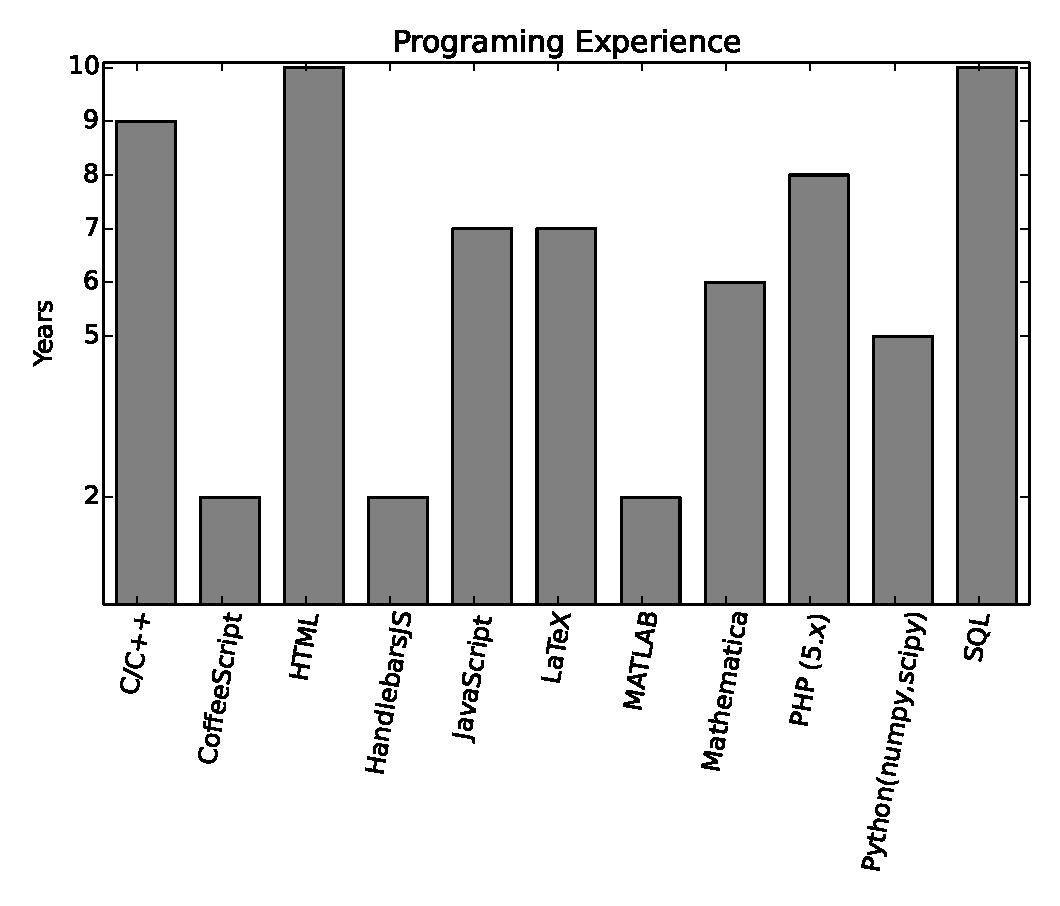
\includegraphics[trim=0.5cm 2.5cm 0 3cm, width=1.0\linewidth]{lanexp} 
				\end{subfigure}
				\begin{subfigure}{.5\textwidth}
  					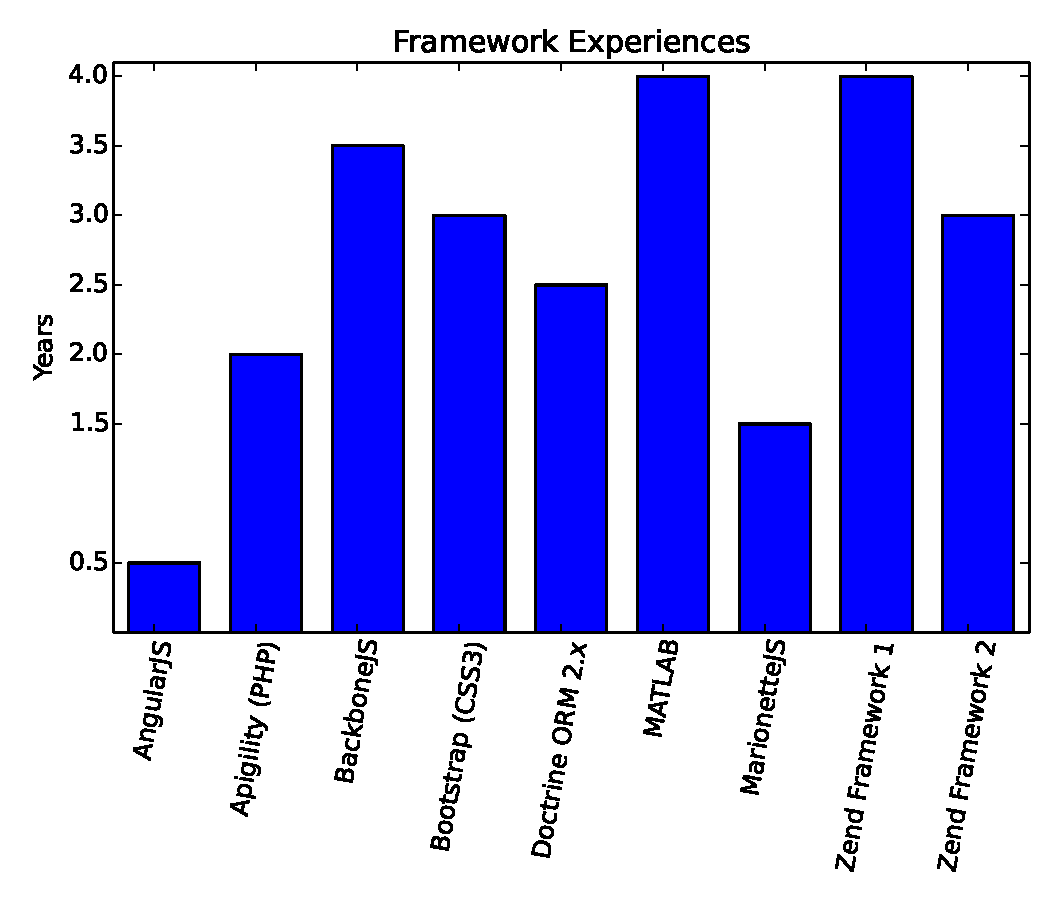
\includegraphics[ width=1.0\linewidth]{frameworkexp}									\end{subfigure}
			\end{figure}
	\end{description} % End Skills list
\resheading{Education}
	\begin{itemize}
		\item
		       Astrophysical Sciences and Technology (Graduate Studies)  \ressubheading{\href{http://www.rit.edu}{Rochester Institute of Technology (RIT)}}{2009 -- 2013}{\href{http://www.rit.edu/cos/astrophysics/}{The School of Mathematical Sciences }}{}
				{ \footnotesize
					\begin{itemize}
						\resitem{Specialized in computational physics }				
					\end{itemize}
				}
                       \item Bachelor of Science in Physics (BS)
                        \ressubheading{\href{http://www.utb.edu}{The University of Texas at Brownsville (UTB)}}{2008}{\href{http://www.phys.utb.edu/}{Department of Physics and Astronomy}}{}

			\item Professional Diploma in Computer Science (BCS)
                        \ressubheading{\href{http://www.bcs.org/}{British Computer Society }}{2001}{\href{http://www.phys.utb.edu/}{}}{}
            \end{itemize} % End Education list
\resheading{\href{http://arxiv.org/a/peiris_p_1.html}{Scientific Publications }}
\label{sec:publications}

\begin{itemize}

\item [*] \href{http://arxiv.org/abs/1504.05890} {A Model-Based Cross-Correlation Search for Gravitational Waves from Scorpius X-1 (arXiv:1504.05890)}

%\item [2] \href{http://arxiv.org/abs/1205.2216} {Search for gravitational waves associated with gamma-ray bursts during LIGO science run 6 and Virgo science runs 2 and 3 (arXiv:1205.2216)}

%\item [3] \href{http://arxiv.org/abs/1202.2788}{All-sky search for gravitational-wave bursts in the second joint LIGO-Virgo run (arXiv:1202.2788)}


%\item [4] \href{http://arxiv.org/abs/1201.5999}{Search for Gravitational Waves from Intermediate Mass Binary Black Holes (arXiv:1201.5999)}


%\item [5] \href{http://arxiv.org/abs/1112.5004}{Upper limits on a stochastic gravitational-wave background using LIGO and Virgo interferometers at 600-1000 Hz (arXiv:1112.5004)}

%\item [6] \href{http://arxiv.org/abs/1112.5004}{Search for Gravitational Waves from Low Mass Compact Binary Coalescence in LIGO's Sixth Science Run and Virgo's Science Runs 2 and 3 (arXiv:1111.7314)}

%\item [7] \href{http://arxiv.org/abs/1110.0208}{All-sky Search for Periodic Gravitational Waves in the Full S5 LIGO Data (arXiv:1110.0208)}

\end{itemize}

I am particularly proud of the above publication. You can see the list of my scientific publication by following the link (\href{http://arxiv.org/a/peiris_p_1.html}{http://arxiv.org/a/peiris\_p\_1.html})  to the distribution server for research articles at Cornell University.
\end{document}